\documentclass[a4paper, twoside, 12pt]{report}

\usepackage{titlesec}
\usepackage{polski}
\usepackage{graphicx}
\graphicspath{ {./images/} }
\usepackage[utf8]{inputenc}
\usepackage[margin=25mm]{geometry}
\usepackage{indentfirst}
\linespread{1}
\titleformat*{\section}{\fontsize{14pt}{2}\bfseries}
\titleformat*{\subsection}{\fontsize{13pt}{2}\bfseries}
\titleformat*{\subsubsection}{\fontsize{13pt}{2}\bfseries}
\usepackage[T1]{fontenc}
\usepackage{mathptmx}



\begin{document}

\title{Ukryte kanały transmisji danych w sieciach komputerowych}
\author{Marcin Szachun}
\maketitle


\begin{abstract}
    Zapewnienie bezpiecznej komunikacji było od zawsze jednym z największych
    problemów telekomunikacji. Tradycyjnie bezpieczna transmisja była możliwa
    dzięki wykorzystaniu kryptografii. Wraz z zastosowaniem coraz bardziej wysublimowanych
    ataków na algorytmy kryptograficzne, oprócz udoskonalania tych algorytmów rozpoczęto
    poszukiwania innych sposobów zabezpieczania wymienianych informacji. Jednym
    z proponowanych rozwiązań jest steganografia, nauka zajmująca się opracowywaniem
    metod komunikacji, w sposób utrudniający wykrycie istnienia wymienianych komunikatów.
    Niniejsza praca zawiera krótki przegląd przykładowych sposobów
    realizacji kanałów ukrytych na potrzeby transmisji danych w sieciach komputerowych.
    W głównej części pracy wysuwana jest propozycja stworzenia kanału ukrytego, opartego na ukrywaniu
    danych w długości pakietów protokołu UDP przesyłanych kanałem podstawowym.
    Przedstawiony protokół kanału ukrytego wspiera zarówno agregację jak i fragmentację
    wiadomości podstawowych w celu transmisji wiadomości ukrytych. Przeprowadzone
    zostały szczegółowe badania parametrów jakościowych takiego kanału w zależności
    od przyjętych parametrów protokołu kanału ukrytego. Podjęta została również
    analiza ingerencji w kanał podstawowy oraz wykrywalności kanału zorganizowanego w taki sposób.
    Dokument zawiera wskazówki doboru parametrów protokołu kanału ukrytego, w taki sposób, aby
    zminimalizować jego ingerencję w kanał podstawowy. Ponadto zostały podane inne
    wskazówki pozwalające zmniejszyć szansę na wykrycie faktu, że kanał ukryty jest
    używany. Zaprezentowano również przykładowe środowiska, w których przedstawiony
    kanał ukryty może być wykorzystywany.
\end{abstract}

\tableofcontents

\listoffigures

\chapter{Cel i zakres pracy}
    Celem niniejszej pracy jest przedstawienie zaprojektowanego protokołu kanału
    ukrytego, działającego w sieciach komputerowych i  opartego o ukrywanie wiadomości za pomocą długości pakietów UDP
    zawierających wiadomości podstawowe. W ramach tego celu zostaną wykonane:
    \begin{itemize}
        \item prezentacja steganografii, nauki o ukrywaniu wiadomości w różnego rodzaju nośnikach,
            oraz steganoanalizy, nauki o wykrywaniu, wraz z ewentualnym niszczeniem kanałów
            ukrytej komunikacji, wraz z najczęściej używanymi pojęciami
        \item przedstawienie przykładowych, innych niż zaproponowany w pracy,
            sposobów organizacji kanałów ukrytych, z zakresu steganografii sieciowej,
            z wykorzystaniem różnego rodzaju protokołów komunikacyjnych
        \item zaprezentowanie projektu protokołu kanału ukrytego, ukrywającego
            wiadomości ukryte za pomocą długości pakietów protokołu UDP, wraz
            z opisem parametrów otrzymanego protokołu, oraz wyjaśnieniem pojęć
            użytych do jego opisu
        \item przeprowadzenie badań czynników wpływających na średnie opóźnienie
            w odbiorze wiadomości podstawowych i ukrytych, wynikających z wykorzystania
            przedstawionego kanału ukrytego,, wraz z analizą wniosków
            z nich płynących
        \item przeprowadzenie analizy wykrywalności zaproponowanego kanału ukrytego,
            wraz z zaproponowaniem sposobów jej zmniejszenia
    \end{itemize}

\chapter{Wstęp teoretyczny}
    \section{Steganografia}
        \subsection{Podstawowe pojęcia}
        \emph{Steganografia} jest to nauka o przesyłaniu komunikatów w taki sposób, aby
        osoba mająca dostęp do kanału, którym prowadzona jest transmisja komunikatów
        nie była w stanie zorientować się, że przesyłane komunikaty istnieją.
        Do ukrycia wiadomości ukrytych wykorzystuje się 
        \emph{nośniki steganograficzne}\cite{STEGANOGRAFIASIECIOWAART}.
        Jednymi z najczęściej wykorzystywanych nośników są multimedia takie jak
        obrazy oraz dźwięki. Poprzez modyfikację własności nośnika możliwe jest
        ukrycie w nim \emph{wiadomości ukrytej}. Pomimo, że osoba postronna ma
        dostęp do zmodyfikowanego nośnika z zawartą w nim wiadomością ukrytą,
        czyli tak zwanym \emph{steganogramem}, nie wzbudza on w niej podejrzeń,
        że może on przenosić jakieś ukryte dane. Procedurę mówiącą w jaki sposób
        zmodyfikować właściwości nośnika aby ukryć w nim wiadomość opisuje
        \emph{algorytm steganograficzny}. W ramach algorytmu steganograficznego
        opisuje się także przekształcenie odwrotne, które musi
        wykonać odbiorca steganogramu, w celu odzyskania wiadomości ukrytej.
        Opcjonalnie zachowanie algorytmu steganograficznego może być modyfikowane przy pomocy specjalnego
        parametru, tak zwanego \emph{klucza}.  Dla takiej samej wiadomości ukrytej i nośnika
        wykorzystywanego do jej ukrycia, różne wartości klucza powodują, że algorytm
        w inny sposób modyfikuje właściwości nośnika, w rezultacie dając inne
        steganogramy.

        \subsection{Zastosowanie}
        Steganografia nie jest nową nauką. Pierwsze wzmianki o zastosowaniu technik
        służących do ukrywania informacji pochodzą ze starożytnej Grecji.\cite{STEGANOGRAPHYINTRO}
        W tamtych czasach wykorzystywane one były do przesyłania wiadomości
        podczas pobytu w niewoli, bądź w celu planowania różnego rodzaju spisków.

        Obecnie zainteresowanie steganografią rośnie i znajduje ona coraz więcej
        zastosowań w różnych dziedzinach. Podstawowym celem w jakim stosowana jest
        steganografia jest zabezpieczenie przed dostępem do wiadomości osób do tego nie
        upoważnionych. W większości przypadków, wykorzystywana jest do tego
        kryptografia. W odróżnieniu od steganografii, kryptografia nie stara się
        ukryć faktu istnienia wiadomości, tylko za pomocą algorytmów kryptograficznych
        przekształcić ją w taki sposób, aby nie możliwe było jej odczytanie bez posiadania
        klucza. Osoba, która przechwyci zaszyfrowaną komunikację nie może co prawda
        odczytać komunikatów, jednak jest dla niej oczywiste, że nadawca i odbiorca
        komunikują się ze sobą i że jakaś tajna wiadomość, nie przeznaczona dla niej,
        istnieje.\cite{DIGITALWATERMARKING} Cecha ta sprawia, że kryptografii nie
        powinno się stosować tam, gdzie konieczne jest zachowanie w tajemnicy
        faktu istnienia wiadomości lub faktu prowadzenia komunikacji. Jako przykład
        można tutaj podać komunikację pomiędzy różnego rodzaju służbami specjalnymi
        podczas organizacji i prowadzenia akcji specjalnych, na przykład odbijania zakładników.
        W przypadku gdyby przestępcy, przechwyciliby zaszyfrowaną komunikację
        pomiędzy oddziałami, mogliby nabrać podejrzeń, jeśli natomiast przechwycona
        zostałaby niezaszyfrowana, niewinnie wyglądająca komunikacja, nie powinna ona
        wzbudzić żadnych obaw. Steganografia wykorzystywana jest również do prowadzenia
        działań wywiadowczych i anty wywiadowczych. Szpiedzy wykorzystują ją do
        bezpiecznej i nie wzbudzającej podejrzeń komunikacji z macierzystą agencją
        wywiadowczą.

        Kryptografia nie może również zostać wykorzystana w miejscach, w których
        nie pozwala na to prawo.\cite{CRYPTOGRAFYLAW} W takich krajach wszelkie
        zaszyfrowane wiadomości mogą być niszczone przez instytucje zajmujące się
        cenzurą. Steganografia jest w takim
        wypadku jedynym środkiem umożliwiającym bezpieczną komunikację. Ponadto
        dzięki jej zastosowaniu, możliwe jest użycie zabronionych algorytmów szyfrujących,
        co dodatkowo zabezpiecza komunikację, ponieważ cenzor nie jest świadomy
        istnienia zaszyfrowanej wiadomości. W niektórych krajach użycie kryptografii
        może być dozwolone, jednak mogą być narzucone ograniczenia, na algorytmy
        kryptograficzne, które mogą być wykorzystywane, lub też na maksymalną
        długość klucza kryptograficznego. Może to rodzić podejrzenia, że ustawodawca
        specjalnie ogranicza dostępne metody kryptograficzne, aby w razie konieczności
        być w stanie złamać i odszyfrować wymieniane wiadomości. Ustawodawca
        może ograniczyć dostępne algorytmy, do własnościowych algorytmów, bądź
        udostępniać jedynie własnościowe implementacje algorytmów kryptograficznych.
        Powoduje to nieufność do udostępnionych rozwiązań, nie tylko ze względu
        na zasadę Kerckhoffsa zgodnie z którą:
        "Algorytm kryptograficzny nie powinien być utrzymywany w sekrecie i nie powinno
        być problemem wykradnięcie go przez wroga".\cite{KERCKHOS}, ale również,
        w świetle doniesień Edwarda Snowdena na temat programów takich jak
        Ballrun\cite{WIKI:BALLRUN}, budzi obawę o możliwość umieszczenia w tych
        algorytmach "tylnych furtek", umożliwiających odszyfrowanie zaszyfrowanych
        nim wiadomości.

        Kolejnym przykładem zastosowanie technik używanych w steganografii jest
        tworzenie znaków wodnych(ang. \emph{watermark}). Jest to dziedzina bardzo zbliżona do steganografii,
        jednak różnica polega na tym, że w przypadku steganografii w nośnej ukrywamy
        informację nie związaną bezpośrednio z samą nośną, natomiast w przypadku znakowania,
        ukryty komunikat w jakiś sposób odnosi się do nośnej. Przykładowym zastosowaniem
        znakowania jest umieszczenie informacji o autorze obrazu w pliku ze zdjęciem.
        Ponadto w przypadku znakowania, istnienie znaku wodnego, nie musi być tajemnicą,
        jednak nadal musi być on "ukryty", to znaczy być zawarty w nośnej, jednak
        nie przeszkadzać w jej odbiorze, na przykład w oglądaniu oznakowanego obrazu.
        Oprócz tego usunięcie znaku wodnego powinno być trudne dla osób do tego nie
        uprawnionych. W przypadku, gdyby druga osoba skopiowała dzieło innej osoby,
        w którym ukryty był znak wodny, może on posłużyć prawowitemu autorowi w
        sądzie do udowodnienia, kto jest prawdziwym autorem.

        Bardzo zbliżonym do znakowania zastosowaniem technik steganograficznych jest
        tworzenie "odcisków palca"(ang. \emph{fingerprinting}). Jest to specjalny
        typ znaku wodnego, unikalny dla każdej kopii dzieła(pliku). Dzięki odciskowi
        palca, możliwe jest zidentyfikowanie osoby winnej, na przykład wycieku informacji
        do mediów, lub też nielegalnie udostępniającej plik w Internecie. W przypadku,
        gdy jeden z nabywców filmu udostępnia go nielegalnie w Internecie, sprzedawca,
        który w każdej sprzedanej kopii umieścił unikany odcisk palca, może porównać
        odcisk palca w udostępnianym pliku, z zapisanymi wcześniej odciskami palców
        w kopiach sprzedanym poszczególnym klientom.

        Techniki ukrywania informacji wykorzystywane są także do rozbudowywania
        istniejących od dawna formatów danych, w celu przechowywania dodatkowych
        danych lub metadanych. Często zdarza się na przykład, że wraz z obrazem
        chcielibyśmy przechowywać jego opis. Dzięki steganografii możemy dodać
        taką zawartość nawet do formatów plików, które nie wspierają natywnie
        przechowywania tego typu danych, nie łamiąc wstecznej kompatybilności z innymi
        programami obsługującymi dany format plików. Przykładem takiego wykorzystania
        steganografii jest przechowywanie opisów zdjęć medycznych, na przykład
        z prześwietleń, w tym samym pliku co obraz.\cite{DISAPPEARINGCRYPTOEMBEDDINGMETDATA}

        \subsection{Przykładowe metody stegnograficzne}
        Jeden z pierwszych historyków greckich Herodot, w swoim dziele "Dzieje"
        opisuje historię starożytnego polityka grackiego Histiajosa, który spiskował
        ze swoim zięciem Arystagorasem, w celu wywołania powstania miast greckich
        przeciw Persom\cite{STEGANOGRAPHYINTRO}. Ponieważ Persowie nie ufali Histiajosowi, musiał on komunikować
        się ze swoim zięciem w sposób sekretny. Według Herodota, wykorzystywał
        on w tym celu swojego najbardziej zaufanego niewolnika, najpierw goląc
        go na łyso, a następnie tatuując mu ukryte wiadomości na skórze głowy.
        Gdy niewolnikowi odrastały włosy, był on wysyłany do Arystagorasa, oficjalnie
        transportując inną, nie związaną ze spiskiem i niewinnie wyglądającą wiadomość.
        Gdy niewolnik docierał do miejsca przeznaczenia, spotykał się Arystagorasem i
        gdy nie było przy nich osób postronnych mówił on o istnieniu wiadomości ukrytej.
        Po ponownym ogoleniu głowy niewolnika Arystagoras zapoznawał się z wiadomością
        od teścia.

        Inną techniką ukrywania wiadomości opisywaną również przez Herodota
        jest wykorzystanie drewnianych tabliczek. Zazwyczaj tabliczki te pokrywane
        były woskiem, w którym można było utrwalić wiadomość, a następnie, gdy
        nie była ona już potrzebna, stopić wosk i otrzymać tabliczkę gotową do
        ponownego użycia. Grek Demaratos chcąc ostrzec Spartę przed atakiem Persów,
        wyrył ostrzeżenie bezpośrednio w drewnie, następnie pokrył je woskiem
        i zapisał na nim niewinnie brzmiącą wiadomość.

        W średniowieczu często stosowane były atramenty sympatyczne, czyli takie,
        które po zapisaniu wiadomości na papierze stawały się niewidoczne, a do
        odczytania ukrytej wiadomości konieczne było "wywołanie" dokumentu. Procedura
        wywoływania była różna w zależności od substancji, która została użyta jako
        atrament sympatyczny. Wśród substancji używanych w tym celu można wymienić:
        mleko, sok cytrynowy, mocz, ocet czy też amoniak. Atramenty sympatyczne
        były nadal wykorzystywane w czasie obu wojen światowych.

        Jedna z ciekawszych technik steganograficznych została zaprezentowana przez
        Gaspari Schotti\cite{NUTYSTEGANOGRAFIA},
        który zaproponował kodowanie liter za pomocą nut. Każdej literze alfabetu
        odpowiadała jedna nuta, różniąca się od innych pod względem wysokości
        dźwięku i czasu jego trwania. Dla osoby nie znającej się na muzyce, tak zakodowana
        wiadomość wygląda na zwykły utwór muzyczny, jednak gdyby zagrać ją na instrumencie
        muzycznym, najprawdopodobniej nie byłyby to miłe uchu dźwięki.

        W czasach, gdy w wielu krajach obowiązywała cenzura, powszechne było ukrywanie
        informacji w tekstach. Odbywało się to poprzez odpowiedni dobór słów,
        z których składał się tekst. Odczytywanie tak ukrytych wiadomości możliwe było
        dzięki, na przykład odczytywaniu drugiej litery każdego ze słów, bądź pierwszej
        litery każdego ze zdań.

        Wspomniano wcześniej, że techniki steganograficzne wykorzystywane są do umieszczania
        odcisków palców w dokumentach. Warto tutaj przytoczyć sztuczkę zastosowaną
        przez Margaret Thatcher, poirytowaną częstymi wyciekami zdjęć tajnych dokumentów
        do prasy. Zażądała ona przeprogramowania oprogramowania do redagowania tych
        dokumentów, w taki sposób, aby w każdej kopii udostępnionej jej współpracownikom,
        poprzez zastosowanie różnych odstępów pomiędzy wyrazami, ukryć informację
        komu udostępniono daną kopię. Dzięki temu, gdy ponownie pojawiły się one w
        prasie, mogła ona zidentyfikować współpracownika odpowiedzialnego za wyciek.\cite{DIGITALWATERMARKING}

        Wraz z rozwojem informatyki i komputerów pojawiły się nowe możliwości
        ukrywania danych. Pojawiło się zainteresowanie wykorzystaniem plików
        multimedialnych na przykład obrazów lub nagrań, jako nośnika dla wiadomości
        ukrytych. Wiąże się to z powstaniem dziedziny zwanej steganografią cyfrową.
        Jednym z najpopularniejszych sposobów wykorzystywanych w tej dziedzinie,
        jest ukrywanie danych poprzez modyfikację najmniej istotnego bitu. Jest
        to metoda wykorzystywana zarówno do plików graficznych\cite{LSBSTEGANGRAPHY},
        jak i dźwiękowych\cite{AUDIOLSBSTEGANGRAPHY}.
        Polega ona na modyfikacji najmniej znaczącego bitu opisującego kolor piksela
        (lub daną próbkę nagrania), w taki sposób, aby ukryć w nim część danych
        ukrytych i aby jednocześnie zmiana w wyglądzie(lub brzmieniu) obraz(nagrania)
        była niedostrzegalna. Tak otrzymany steganogram może być łatwo rozpowszechniany
        w Internecie, a dostęp do niego może mieć duża grupa osób.

        Jednym z najnowszych obszarów steganografii cyfrowej jest steganografia
        sieciowa, której poświęcony został jeden z kolejnych rozdziałów pracy.
        Ponadto praca ta zawiera propozycję organizacji kanału ukrytego, zawierającą
        się właśnie w tym obszarze steganografii.

    \section{Steganoanaliza}
        \subsection{Podstawowe pojęcia}
        Podobnie jak kryptografii towarzyszy kryptoanaliza, tak i steganografii
        towarzyszy nauka zwana \emph{steganoanalizą}. Zajmuje się ona badaniem
        nośników, pod kątem przenoszenia przez nie danych ukrytych, ponadto badane
        są sposoby niszczenia danych ukrytych. W kryptografii system uznaje się
        za \emph{skompromitowany}, gdy kryptologowi uda się odczytać zaszyfrowaną wiadomość.
        Dla steganografii poprzeczka jest podniesiona, do jej skompromitowania wystarczy,
        że dowiedzione zostanie, że wiadomość ukryta istnieje w nośnej, nie jest
        konieczne jej odczytanie. Jeśli ponadto atakującemu uda się odczytać wiadomość
        ukrytą, zwiększa to poziom kompromitacji systemu.

        Wyróżnia się dwie metody prowadzenie steganoanalizy: pasywną i aktywną.
        Celem metody pasywnej jest wykrycie istnienia wiadomości ukrytej. Każdy przekazywany
        przez nadawcę komunikat, jest analizowany pod względem zawierania tajnej wiadomości.
        W przypadku, gdy taka wiadomość zostanie wykryta, komunikacja zostaje przerwana,
        w przeciwnym wypadku, wiadomość jest dostarczana do odbiorcy. Osoba lub system,
        który zajmuje się analizą przesyłanych wiadomości, nazwana jest \emph{agentem(ang. warden)}.
        Steganoanaliza pasywna dzieli się na dwie grupy, \emph{steganoanaliza kierowana(ang. targeted)}, gdy
        atakujący podejrzewa algorytm, lub grupę algorytmów steganograficznych,
        które zostały użyte do ukrycia informacji i jest w stanie dopasować do
        niego sposób prowadzenia analizy, oraz \emph{steganoanalizę ślepą(ang. blind)},
        gdy musi on stosować ogólne sposoby analizy, które są w stanie wykryć różnego
        rodzaju algorytmy steganograficzne. Po wykryciu obecności wiadomości ukrytej,
        agent może przeprowadzić \emph{steganografię śledczą, wywiadowczą(ang. forensic steganalysis)},
        w celu wydobycia treści wiadomości ukrytej. W takim przypadku nie musi on
        blokować komunikacji pomiędzy odbiorcą a nadawcą, co mogłoby spowodować,
        że zorientowali by się oni, że bezpieczeństwo ich komunikacji może być zagrożone,
        a zamiast tego podsłuchiwać wymieniane przez nich wiadomości.

        W przypadku prowadzenie \emph{steganoanalizy aktywnej} agent ma więcej możliwości
        działania. W szczególności może on modyfikować wiadomości przesyłane pomiędzy
        nadawcą a odbiorcą. Jego celem nie koniecznie musi być wykrycie, czy wiadomość
        ukryta istnieje, ale na przykład upewnienie się, że na pewno nie dotrze ona
        do odbiorcy. W związku z tym, nawet jeśli błędnie nie wykryje on wiadomości ukrytej,
        może on modyfikować wiadomość podstawową, starając się usunąć wiadomość ukrytą,
        ale nadal zachowując sens i znaczenie wiadomości podstawowej. Tego typu analiza
        najczęściej skierowana jest przeciwko omówionym wcześniej znakom wodnym,
        oraz cyfrowym odciskom palców.\cite[Rozdział 13]{DIGITALWATERMARKING}

        \subsection{Zastosowanie}
        Wraz ze wzrostem zainteresowania steganografią, steganoanaliza jest wykorzystywana
        coraz częściej, we wszystkich miejscach, gdzie podejrzewane jest stosowanie
        steganografii.

        Wspomniano wcześniej o krajach, które próbują ograniczać
        prawo do wolności słowa swoich obywateli, na przykład poprzez ograniczenia
        wykorzystania kryptografii. Wobec zagrożenia użyciem steganografii, cenzorzy,
        stosują steganoanalizę, w celu wykrycia prób sekretnej komunikacji i jej zapobiegnięciu.
        Ze względu na specyfikę działania cenzora, zazwyczaj używa on steganoanalizy
        aktywnej, aby upewnić się, że jakiekolwiek wiadomości ukryte zostaną zniszczone.

        Steganoanaliza jest powszechnie wykorzystywana w zastosowaniach militarnych.
        Historia wielu wojen pokazuje, że poznanie zawczasu planów, oraz pozycji
        wojsk przeciwnika, pozwala uzyskać nad nim znaczną przewagę. Jako przykład
        można tutaj przytoczyć załamanie wiadomości zaszyfrowanych niemiecką maszyną
        szyfrującą "Enigma", w którym znaczący udział mieli polscy matematycy i kryptolodzy.
        Szacuje się, że dzięki temu II Wojna Światowa trwała około 2 -3 lata krócej
        i ocalone zostało około 30 milinów ludzi. Poprzez niszczenie ukrytych wiadomości wroga,
        w konsekwencji zakłócając komunikację i powodując dezorganizację we wrogich oddziałach,
        również można pogorszyć jego sytuację.
        W związku z tym, wywiad wojskowy wykorzystuje zarówno techniki opracowane w
        ramach steganoanalizy pasywnej, wywiadowczej i aktywnej.

        Niestety możliwość wymiany wiadomości bez wzbudzania podejrzeń bywa nadużywana.
        Oprócz wspomnianych wcześniej legalnych zastosowań, steganografia może
        być wykorzystywana przez organizacje przestępcze oraz terrorystyczne. Podejrzewa
        się, że do zorganizowania ataków na wieże World Trade Center, 11 września 2001 roku,
        terroryści wykorzystywali metody powiązane ze staganografią, a obecnie wykorzystują
        je powszechnie\cite{TERRORISMANDSTEGANOGRAPHY}.
        Powoduje to, że służby zajmujące się utrzymaniem bezpieczeństwa wykorzystują
        steganoanalizę do łapania przestępców, oraz zapobieganiu ich działaniom.

        Najpowszechniejszym zastosowaniem steganoanalizy, podobnie jak kryptoanalizy,
        jest analizowanie oraz ocenianie nowych i już istniejących algorytmów steganograficznych.
        Jak wcześniej wspomniano algorytmy te wykorzystywane są w wielu miejscach,
        a niekiedy bezpieczeństwo zapewniane przez te algorytmy jest kluczowe, jak
        na przykład przy przesyłaniu tajnych wiadomości wojskowych, czy też przy znakowaniu
        utworów. Powoduje to, że poznanie mocnych i słabych stron algorytmów steganograficznych
        jest bardzo ważne. W celu oceny algorytmu, pod uwagę branych jest kilka czynników
        bezpieczeństwo, czyli trudność i ilość pracy jaką trzeba włożyć,
        w badanie steganogramu, aby odkryć istnienie ukrytej wiadomości.
        Ponadto w ramach badania bezpieczeństwa, zazwyczaj sprawdza się, jak ciężko
        jest odczytać treść ukrytej wiadomości, po odkryciu jej istnienia.
        Pojemność, czyli
        ilość informacji, które jest w stanie ukryć algorytm, w pojedynczej jednostce
        nośnika(na przykład w jednym obrazie, lub jednym pakiecie sieciowym). Badane
        jest także jak trudne jest usunięcie informacji ukrytej w steganogramie, przy
        użyciu steganoanalizy aktywnej.

        \subsection{Przykłady zapobiegania wykorzystywaniu steganografii}
        Jak zostało wcześniej wspomniane, do wykrywania i zapobiegania wykorzystaniu stegangrafii
        wykorzystywane są różnego rodzaju techniki opracowane w ramach steganoanalizy.
        Część ataków na algorytmy steganograficzne jest podobna do ataków na
        algorytmy kryptograficzne. Steganografia stara się zapewnić dodatkowe bezpieczeństwo
        poprzez ukrycie wiadomości, w związku z tym jest podatna na dodatkowe ataki.
        Podobnie jak w przypadku kryptografii, im większą ilość danych na temat
        algorytmu steganograficznego i wymienianych wiadomości posiada atakujący,
        tym groźniejsze i bardziej wyrafinowane ataki jest w stanie przeprowadzić.
        Wśród możliwych ataków wyróżniamy\cite{DISAPPEARINGCRYPTOEMBEDDINGMETDATA}:
        \begin{itemize}
            \item atak ze znanym steganogramem - atakujący ma dostęp jedynie do
                steganogramu, ewentualnie pewnej ich kolekcji, przechwyconych poprzez
                podsłuchiwanie komunikacji, na tej podstawie podejmuje on decyzję,
                czy zawierają one wiadomość ukrytą, czy nie, analiza ślepa opiera
                się w tym przypadku o analizę statystyczną steganogramu i poszukiwaniu
                odchyleń od normy lub o badanie zgodności wymienianych wiadomości
                ze standardami(na przykład zgody z oficjalną specyfikacją formatu pliku,
                lub protokołu komunikacyjnego), możliwe jest rozszerzenie
                analizy o próbę odczytania zawartości wiadomości ukrytej, po stwierdzeniu
                jej istnienia
            \item atak ze znanym steganogramem i oryginalnym nośnikiem - w przypadku
                takiego ataku steganoanalityk jest w stanie łatwo wykryć istnienie
                wiadomości poprzez porównanie nośnika ze steganogramem, jednoznacznie
                potwierdza to istnienie wiadomości ukrytej, ponieważ z definicji
                każdy algorytm steganograficzny powoduje modyfikację właściwości
                nośnika, w przypadku tego ataku najczęściej wysiłki skupiają się
                na odczytaniu zawartości wiadomości ukrytej
            \item atak ze znajomością algorytmu steganograficznego - atak ten
                stosowany jest przeciwko algorytmom używającym klucza steganograficznego,
                w celu odczytania zawartości wiadomości ukrytych, klucz steganograficzny
                jest najczęściej ziarnem dla generatora liczb losowych, który z
                kolei kontroluje proces ukrywania wiadomości w nośniku, przeprowadzanie
                takiego ataku przeciw algorytmom nie używającym klucza kryptograficznego
                nie jest konieczne, ponieważ znając algorytm, atakujące może wykrywać i
                odczytywać tajne wiadomości
            \item atak niszczący ukryte wiadomości - jak wspomniano wcześniej, niekiedy
                celem atakującego nie jest wykrycie wiadomości ukrytej, ale upewnienie
                się, że nie dotrze ona do odbiorcy, w tym celu może on poddać steganogram
                procesom takim jak filtrowanie(obrazy, dźwięki, skuteczne przeciwko
                algorytmom ukrywającym dane w najmniej znaczącym bicie), kompresja(bardzo skuteczna
                metoda przeciwko większości algorytmów), konwersja do innego formatu
                bądź użycie innego protokołu komunikacyjnego(skuteczniejsze niż konwersja) lub
                przeformułowanie wiadomości nośnej(na przykład poprzez zapisanie tego samego tekstu
                innymi słowami)
            \item atak zastępujący ukrytą wiadomość - atak stosowany w celu zniszczenia
                wiadomości ukrytej, lub zastąpienia jej wiadomością przygotowaną przez atakującego,
                stosowany, gdy dysponuje on specyfikacją algorytmu steganograficznego,
                polega na zastosowaniu algorytmu ponownie, traktując steganogram jako nośnik
                nowej ukrytej wiadomości, większość algorytmów jest podatna na ten
                atak, ponieważ ukrywają one wiadomość atakującego w taki sam sposób,
                jak oryginalną wiadomość ukrytą, tym samym ją niszcząc
        \end{itemize}


\chapter{Charakterystyka możliwości realizacji kanałów ukrytych w sieciach komputerowych}
    Wraz z rozwojem i coraz powszechniejszym wykorzystaniem komputerów i sieci
    komputerowych, prężnie rozwija się dziedzina steganografii zwana steganografią
    sieciową. Do tworzenia kanałów umożliwiających transmisję wiadomości ukrytych
    wykorzystuje ona protokoły komunikacyjne i wpływa na ich działanie. W kontekście
    steganografii sieciowej warto wyróżnić zasługi polskich naukowców z Politechniki
    Warszawskiej, którzy wiele wnieśli w rozwój tej nauki\cite{STEGANOGRAFIASIECIOWAART}.

    Protokoły komunikacyjne są zazwyczaj
    precyzyjnie specyfikowane, na przykład w dokumentach RFC, jednak nawet najdokładniejsza
    specyfikacja nie jest w stanie pokryć wszystkich przypadków brzegowych. Powoduje
    to, że w niektórych miejscach specyfikacja pozostawia swobodę implementacji protokołu,
    co w dalszej kolejności powoduje występowanie różnic pomiędzy konkretnymi
    implementacjami, na przykład pomiędzy różnymi systemami operacyjnymi. Ponadto
    w niektórych systemach implementacja protokołów może być okrojona, na przykład
    ze względu na ograniczone zasoby sprzętowe. Te czynniki
    powodują, że pojawia się okazja do nadużyć i wykorzystania niespójności do organizowania
    kanałów ukrytych.

    Mnogość istniejących protokołów pozwala na tworzenie różnorodnych protokołów
    kanałów ukrytych, dostosowanych do konkretnych warunków komunikacyjnych.
    Mogą być w tym celu wykorzystywane protokoły ze wszystkich warstw modelu
    ISO/OSI, chociaż wykorzystanie niektórych warstw może być trudne, lub wiązać
    się z dużym wysiłkiem(na przykład dla warstwy fizycznej lub warstwy danych -
    implementacja dedykowanych sterowników urządzeń sieciowych). Umożliwia to
    też budowę dużych systemów steganograficznych wykorzystujących jednocześnie
    kilka kanałów ukrytych, zorganizowanych na poziomie różnych warstw modelu ISO/OSI.
    Zastosowanie kilku kanałów ukrytych stosowanych na przemian, może pomóc w zmniejszeniu
    wykrywalności całego systemu, poprzez minimalizowanie wywieranego wpływu na pojedynczy
    nośnik(protokół komunikacyjny). Wybór warstwy sieciowej, w której działa kanał ukryty
    ma wpływ między innymi na prawdopodobieństwo przypadkowego usunięcia wiadomości
    ukrytej w trakcie transmisji(na przykład poprzez budowę nowego pakietu na podstawie
    pakietu oryginalnego w czasie trasowania).

    W dalszej części rozdziału przedstawiono podział steganografii sieciowej
    oraz zaprezentowane przykładowe kanały ukryte, charakterystyczne dla danej
    dziedziny.
    \section{Poprzez modyfikację pakietów} \label{MODYFIKACJAPAKIETOW}
        \subsection{Wykorzystanie nieużywanych pól nagłówków}
        Nie tylko wspomniane wcześniej rozbieżności pomiędzy poszczególnymi
        implementacjami powodują powstanie możliwości organizacji kanałów ukrytych.
        Często zdarza się, że protokoły komunikacyjne wymagają rozbudowy o nowe,
        funkcjonalności, o których nie pomyśleli, bądź nawet nie byli świadomi
        ich twórcy na etapie projektowania. W momencie, gdy protokół jest obecny
        na rynku od dawna i jest szeroko używany(dokument RFC opisujący protokół TCP
        powstał w 1981 roku\cite{TCPRFC}), wprowadzanie do niego drastycznych zmian,
        powodujących niekompatybilność z istniejącymi implementacjami, nie jest
        najlepszym pomysłem. W związku z tym, autorzy protokołów często wprowadzają
        do nagłówków tych protokołów nadmiarowe pola, zarezerwowane do wykorzystania
        w przyszłości. Takie pola nie są wykorzystywane przez aktualne implementacje
        protokołów, co pozwala na wykorzystanie ich w celu transmisji ukrytych danych.

        Jeden z najpopularniejszych protokołów komunikacyjnych używany do niezawodnej
        transmisji danych - TCP, jest przykładem protokołu zawierającego pola zarezerwowane(Rys. \ref{TCPHEADER}).
        Wykorzystanie tego pola pozwala na stworzenie kanału ukrytego pozwalającego
        na transmisję 6 bitów tajnych danych w każdym pakiecie TCP. W przypadku protokołu
        IP, który jest głównym protokołem wykorzystywanym w Internecie, możemy wykorzystać: pole
        opisujące używaną wersję protokołu(4 bity), nie zarejestrowane wartości pola Typ Usługi(2 bity),
        oraz pierwszy bit pola Flagi(1 bit)(Rys. \ref{IPHEADER})\cite{IPRFC}.

        Liczba bitów danych
        możliwych do ukrycia w pojedynczym pakiecie, nie robi może wrażenia, jednak biorąc
        pod uwagę intensywność wykorzystania tych protokołów, można w ten sposób
        stworzyć kanały ukryte o dużych przepustowościach. Inną zaletą kanałów organizowanych
        w ten sposób jest prostota implementacji. Niestety ogromną wadą jest stosunkowa
        łatwość wykrycia. Nawet pasywny warden jest w stanie łatwo wykryć istnienie wiadomości
        ukrytej, poprzez sprawdzanie zgodności zawartości wymienionych wcześniej pól
        nagłówka ze specyfikacją protokołu. Zazwyczaj jest w niej wyraźnie napisane,
        jaką wartością powinny być wypełnione pola zarezerwowane(najczęściej jest to 0).
        Każde odstępstwo od specyfikacji może być traktowane jako podejrzane. Nawet biorąc
        pod uwagę, przytoczony wcześniej argument o niezgodności implementacji protokołów
        ze specyfikacją, zazwyczaj wartość wpisywana przez systemy operacyjne do
        zarezerwowanych pól nagłówków jest stała.

        \begin{figure}[h]
                \centering
                % source: http://intronetworks.cs.luc.edu/current/html/_images/tcp_header.png
                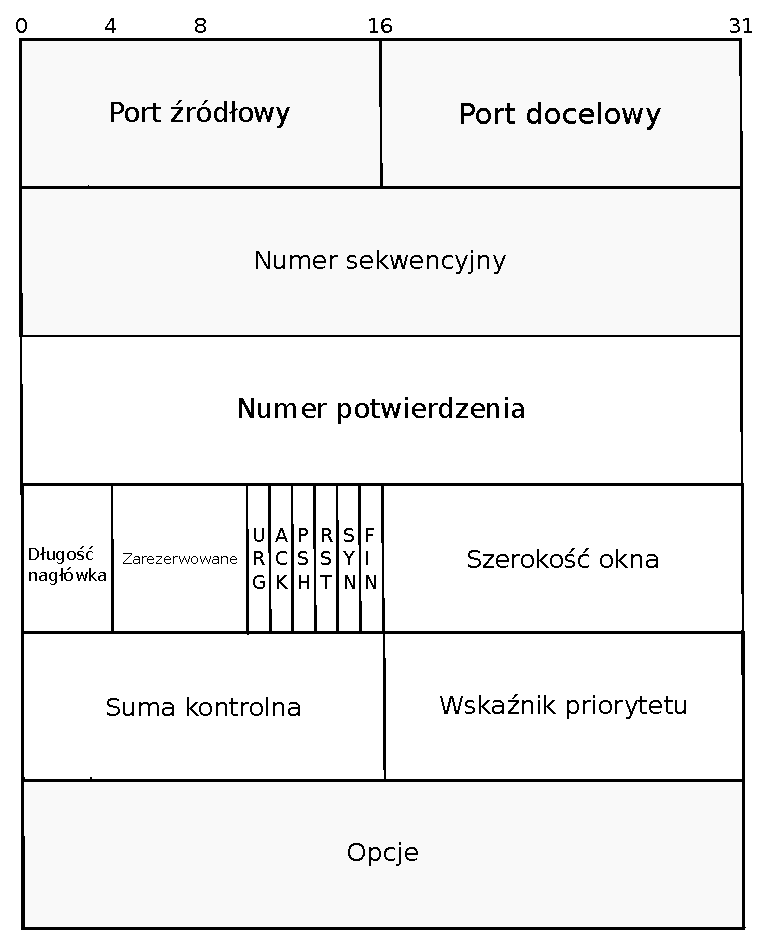
\includegraphics{tcp_header}
                \caption{Format nagłówka protokołu TCP}
                \label{TCPHEADER}
        \end{figure}
        \begin{figure}[h]
                \centering
                % source: http://ps-2.kev009.com/wisclibrary/aix51/usr/share/man/info/en_US/a_doc_lib/aixbman/commadmn/figures/comma35.jpg
                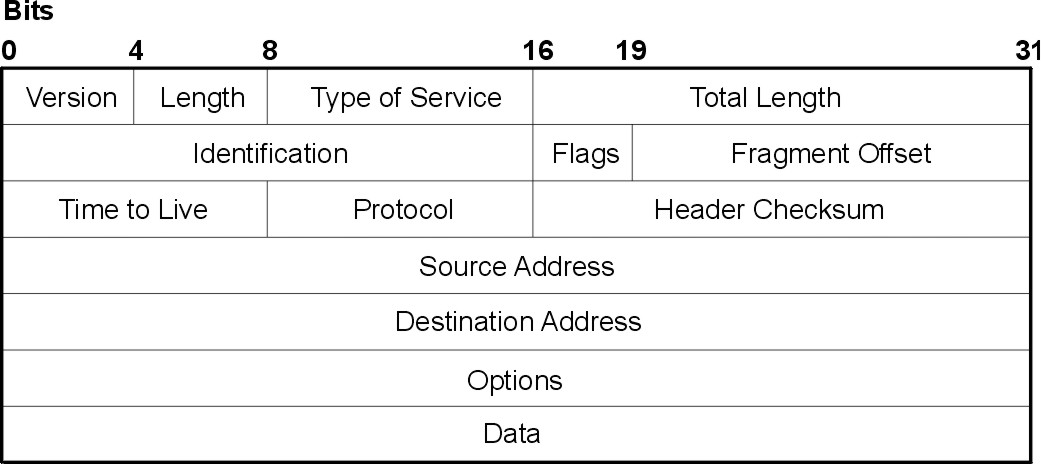
\includegraphics{ip_header}
                \caption{Format nagłówka protokołu IP}
                \label{IPHEADER}
        \end{figure}
        \subsection{Wykorzystanie dopełnienia pakietów}
        Kolejnym sposobem, który można wykorzystać do tworzenia kanałów ukrytych
        jest wykorzystanie dopełnienia. Wykorzystanie dopełnienia przez protokół komunikacyjny
        może być konieczne z kilku powodów. Niektóre algorytmy kryptograficzne, w szczególności
        tak zwane szyfry blokowe, operują na stałym z góry określonym fragmencie danych,
        to znaczy bloku. Taki algorytm nie jest w stanie pracować z danymi, których
        rozmiar nie jest równy rozmiarowi bloku, w związku z tym jeśli długość
        danych zawartych w pakiecie nie jest wielokrotnością długości bloku
        algorytmu używanego do szyfrowania, muszą one zostać uzupełnione, aby możliwe
        było zaszyfrowanie całego pakietu. Taka sytuacja występuje w protokołach,
        które wykorzystują szyfrowanie, na przykład IPSec\cite{IPSECPADDING}.

        Dopełnienie pakietu jest konieczne, gdy protokół zakłada, z góry ustaloną długość
        całego pakietu, lub któregoś z pól nagłówka. Takie założenia spotykane są
        w protokołach, w których można z dużą dokładnością z góry przewidzieć jaką długość
        będą miały transmitowane dane. W przypadku, gdy długość danych może oscylować
        wokół przewidzianej wartości, należy założyć długość pakietu(nagłówka)
        nieco większą niż oszacowana. Gdy długość danych do transmisji jest krótsza niż
        założona długość pakietu(nagłówka), konieczne jest zastosowanie dopełnienia.

        Niekiedy, dopełnienie stosuje się w celu dopasowania długości pola nagłówka,
        do długości słowa maszynowego używanego przez dany system komputerowy. Może
        to w istotny sposób ułatwić implementację sprzętową danego protokołu, lub
        przyspieszyć jego działanie. Ponadto nawet programowe implementacje zyskują
        na szybkości, ponieważ komputery są zoptymalizowane pod względem operowania
        na danych o długości będącej wielokrotnością długości słowa maszynowego.

        Podobnie jak w przypadku pól nieużywanych, teoretycznie specyfikacja
        mówi jaką wartością powinno odbywać się dopełnianie pakietów, co więcej,
        w przypadku dopełniania pakietów dla algorytmu kryptograficznego, zastosowanie
        nieodpowiedniego dopełnienienia może mieć wpływ na bezpieczeństwo szyfrogramu(złe dopełnienie narażone
        jest na atak "padding oracle attack"). Różnice w implementacji protokołów
        i sterowników urządzeń sieciowych, powodują, że dopełnienie można wykorzystać,
        jako miejsce ukrycia danych\cite{PADSTEG}

        Również tak jak w przypadku wykorzystania zarezerwowanych pól nagłówka,
        wykrycie tego rodzaju danych ukrytych może zostać sprowadzone do testowania
        zgodności przesyłanych pakietów ze specyfikacją protokołu. Wcześniej wspomniane
        wykorzystanie wielu protokołów z różnych warstw sieciowych, pozwala zmniejszyć
        prawdopodobieństwo wykrycia ukrytych wiadomości. Przykład implementacji
        takiego kanału ukrytego przedstawiono w \cite{PADSTEG}

        \subsection{Ukrywanie danych w pakietach celowo uszkodzonych} \label{USZKODZONEPAKIETY}
        Obecnie popularne staje się wykorzystanie mechanizmów zapewniania niezawodności
        transmisji do organizacji kanałów ukrytych. Chodzi tutaj o mechanizmy
        takie jak odrzucanie i retransmisja uszkodzonych pakietów. Przykładem wykorzystania takich
        mechanizmów jest umyślne tworzenie pakietów, w których suma kontrolna w nagłówku
        nie zgadza się z sumą kontrolną obliczoną dla treści wiadomości.

        Teoretycznie możliwe są dwa
        sposoby organizacji kanałów ukrytych oparte na tym pomyśle. Pierwszy z nich polega na umieszczeniu
        danych ukrytych w polu nagłówka, w którym zwykle znajduje się suma kontrolna,
        jednak nie ma on praktycznego zastosowania, ze względu, na małą przepływność
        kanału ukrytego i stosunkowo łatwą wykrywalność(transmisja dużej ilości
        danych ukrytych znacząco pogarsza jakość obsługi w kanale podstawowym).

        Inny pomysł polega
        na umieszczeniu danych ukrytych w polu danych pakietu, i sfałszowaniu sumy
        kontrolnej. W takiej sytuacji pakiet wygląda na uszkodzony, w związku z tym
        dla podsłuchującego i dla odbiorcy wiadomości podstawowych wydaje się
        on nie przenosić żadnych użytecznych danych. Odbiorca wiadomości ukrytych,
        widząc, że to właśnie w takich pakietach znajdują się wiadomości ukryte,
        może je odczytać. Kanały ukryte oparte na takiej zasadzie, są w stanie
        zapewnić dużą przepływność, należy jednak uważać, aby liczba wprowadzonych
        uszkodzonych pakietów mieściła się w granicach zdrowego rozsądku, zbyt duża
        ich liczba może przyczynić się do wzrostu wykrywalności kanału. Do wad takiego
        rozwiązania należy zaliczyć brak możliwości wykorzystania kanału, jeśli do
        komunikacji pomiędzy nadawcą a odbiorcą konieczne jest wykorzystanie pośrednika(na przykład routera).
        Jest to spowodowane tym, że zazwyczaj każdy z węzłów pośredniczących w transmisji
        dokonuje kontroli poprawności pakietu(sprawdza sumę kontrolną) i nie przekazuje
        dalej pakietów uszkodzonych.

        Wykorzystanie celowo uszkodzonych pakietów najlepiej sprawdza się w
        sieciach, w których do naturalnych uszkodzeń pakietów, nie związanych z
        istnieniem kanału ukrytego, dochodzi stosunkowo często. W związku z tym
        świetnie nadają się sieci bezprzewodowe oraz takie, w których występują
        częste zakłócenia. Przykład implementacji kanału ukrytego, wykorzystującego
        ukrywanie informacji w polu danych uszkodzonych pakietów, w sieci WIFI
        został opisany w \cite{HICCUPS}

    \section{Poprzez modyfikację właściwości strumienia pakietów} \label{MODYFIKACJASTRUMIENIA}
        \subsection{Poprzez manipulację prędkością transmisji}
        Ten sposób organizacji polega na modulacji prędkości transmisji danych
        pomiędzy nadawcą a odbiorcą, w zależności od danych ukrytych, które mają
        być transmitowane. Należy zauważyć, że w przeciwieństwie do poprzednich
        metod, tutaj nie następuje żadna ingerencja, w dane ani nagłówek pakietu.
        Odróżnia to metody przedstawione w tej części rozdziału, od poprzednio
        przedstawionych.

        W celu organizacji kanału ukrytego wyznaczane są odpowiednie zakresy prędkości, oraz ich
        interpretacja. Odbiorca co ustalony czas, dokonuje próbkowania prędkości
        transmisji. Odczytana wartość jest porównana z umówionymi wcześniej zakresami,
        w zależności, w którym z tych zakresów jest ona zawarta, interpretowane jest to
        jako otrzymanie bitu 1, 0 lub brak komunikatu. Rola tych przedziałów jest analogiczna
        do przedziałów kwantyzacji, używanych do kwantyzacji sygnału analogowego.

        Przepływność takiego kanału ukrytego jest pochodną wybranej przez rozmówców
        częstotliwości próbkowania oraz liczby przedziałów kwantyzacji. Pojawia się
        problem doboru długości przedziałów kwantyzacji, za pomocą których wykonywana
        jest interpretacja wartości
        prędkości chwilowej. Muszą być one na tyle długie, aby uwzględniać naturalnie
        występujące w sieciach komputerowych opóźnienia oraz przeciążenia, które wpływają
        na chwilową wartość prędkości transmisji. Z drugiej strony, zbyt długie przedziały
        mogą spowodować, że do transmisji danych ukrytych wymagana będzie duża ilość danych
        podstawowych. Ponadto środki przedziałów należy dostosować do natężenia
        napływu wiadomości podstawowych. Możliwe jest wyznaczenie większej ilości
        przedziałów kwantyzacji, co umożliwia transmisję więcej niż jednego bitu w pojedynczym
        okresie próbkowania.

        Przedstawione problemy powodują, że tego typu kanały muszą być dokładnie
        skonfigurowane pod kątem konkretnej sieci komputerowej, w której będą wykorzystywane.
        Zastosowanie takich kanałów w niestabilnych środowiskach sieciowych(częste zmiany
        opóźnień, lub natężenia napływu danych) jest znacznie utrudnione. Należy jednak
        zauważyć, że po dokładnym skonfigurowaniu oraz przeprowadzeniu dokładnych
        pomiarów opóźnień, kanały ukryte zorganizowane w ten sposób można z powodzeniem
        stosować, nawet wtedy, gdy do komunikacji konieczne jest korzystanie z węzłów pośrednich.
        Węzły pośrednie, o ile zachowują się deterministycznie, nie zmieniają znacznie wcześniej
        zmierzonych wartości opóźnienia oraz prędkości transmisji.

        TODO: TU BĘDZIE OBRAZEK(wykres zależności prędkości transmisji od czasu, z
        oznaczonymi przedziałami kwantyzacji prędkości transmisji, oraz okresami
        próbkowania).

        \subsection{Poprzez manipulację opóźnieniem pakietów}
        Sposobem podobnym do poprzedniego jest interpretacja opóźnień pakietów,
        jako fragmenty pochodzące z danych ukrytych.\cite{IPDELAYCHANNEL} Ten sposób nie wymaga jednak próbkowania,
        ponieważ opóźnienie(rozumiane tutaj jako okres czasu pomiędzy odebraniem dwóch
        kolejnych pakietów), może być precyzyjnie obliczone. Nadal jednak potrzebna
        jest kwantyzacja, ze względu na wpływa warunków zewnętrznych, takich jak przeciążenia,
        na opóźnienie pakietów. Nadawca umyślnie wydłuża lub skraca czas pomiędzy
        wysłaniem kolejnych pakietów, w zależności od fragmentu danych ukrytych,
        które chce przetransmitować. Odbiorca po odebraniu pakietu oblicza czas jaki
        upłynął od odebrania poprzedniego pakietu, następnie
        interpretuje opóźnienie jako fragment wiadomości ukrytej korzystając z
        przedziałów kwantyzacji.

        Przepływność tak uzyskanego kanału zależy od długości i ilości wybranych
        przedziałów kwantyzacji. W związku z tym, jest ona niższa od możliwej do
        uzyskania przy pomocy wcześniej przedstawionego sposobu, ze względu na brak
        możliwości regulacji okresu próbkowania, który jest tutaj nieobecny. Poza tą różnicą, oba sposoby mają
        wiele wspólnego. Podobnie jak w poprzednim przypadku, wyznaczenie długości
        przedziałów kwantyzacji powinno być poprzedzone zbadaniem opóźnień występujących
        naturalnie w środowisku sieciowym, ponieważ nakładają się one na opóźniania
        wprowadzone przez nadawcę. W związku z tym taki kanał ukryty również wrażliwy jest
        na nagłe zmiany charakterystyk pracy sieci komputerowej, jednak w mniejszym
        stopniu niż kanał oparty na modulacji prędkości transmisji. Równie dobrze
        nadaje się on do komunikacji, gdy pomiędzy odbiorcą a nadawcą znajdują się
        węzły pośredniczące.

        Zaletą obu przedstawionych w tej sekcji protokołów komunikacyjnych,
        jest możliwość wykorzystania szerokiego zestawu protokołów jako
        źródeł wiadomości podstawowych. Przedstawione techniki są ogólne i
        nie stawiają żadnych wymagań protokołowi, który zostanie wykorzystany jako
        nośnik(brak wymagań co do określonych pól nagłówka, oraz co do typu transportowanych danych).
        W związku z tym, jako źródło wiadomości podstawowych może być wykorzystany
        praktycznie każdy protokół, pod warunkiem odpowiedniego skonfigurowania
        protokołu kanału ukrytego.


    \section{Podejścia hybrydowe}
        \subsection{Ukrywanie danych w pakietach protokołów strumieniowej transmisji danych}
        W celu połączenia zalet podejść przedstawionych w sekcjach
        \ref{MODYFIKACJAPAKIETOW} i \ref{MODYFIKACJASTRUMIENIA}, oraz wyeliminowania
        ich wad, stworzono kanały steganograficzne, wykorzystujące jednocześnie obie te
        techniki. Takie kanały modyfikują jednocześnie pojedyncze pakiety sieciowe,
        jak i właściwości strumienia pakietów. Dzięki temu, można przesyłać tajne wiadomości,
        nawet do innych sieci komputerowych, z wykorzystaniem pośrednich węzłów sieciowych,
        jednocześnie eliminując dużą zależność protokołu kanału ukrytego od warunków
        panujących w środowisku sieciowym. Ceną, którą należy zapłacić za kanał
        ukryty tej klasy, jest niewielka liczba protokołów, które można wykorzystać
        jako kanał podstawowy. Najczęściej wykorzystywaną klasą protokołów są
        protokoły strumieniowej transmisji danych, wykorzystywane między innymi
        w aplikacjach VOiP, lub strumieniujących multimedia(muzykę, filmy).

        W pracy \cite{VOIPSTEGANOGRAPHY} w celu organizacji kanału ukrytego wykorzystany
        jest protokół RTP(Real-Time Transfer Protocol), jako przykład aplikacji
        wykorzystującej ten protokół wybrano aplikację typu VOiP. W tego typu aplikacjach,
        jeśli odbiorca odbierze pakiet, który jest znacznie opóźniony w stosunku
        do innych pakietów, uznaje się, że informacje w nim zawarte są bezwartościowe,
        ponieważ jest za późno, aby użyć ich do procedury rekonstrukcji głosu.
        Zastosowane przez autorów podejście opiera się na celowym opóźnianiu pakietów
        zawierających dane ukryte, zapisane w polu danych pakietu.
        Odbiorca wiadomości podstawowych odbierając pakiet
        opóźniony, odrzuca go, jednak odbiorca wiadomości wiedząc, że to właśnie
        w nim znajduje się ukryta wiadomość, może ją odczytać.

        Pakiet zostaje rozpoznany jako opóźniony, nie tylko ze względu na celowe
        oczekiwanie z jego wysłaniem przez nadawcę, ale również ze względu
        na umieszczenie sfałszowanego czasu wysłania pakietu w odpowiednim
        polu nagłówka(pole Timestamp). Dzięki temu kanał staje się mniej zależny
        od warunków i opóźnienia naturalnie występującego w sieci komputerowej.

        Jak widać w celu realizacji kanału modyfikowany jest zarówno pakiet(pole danych,
        pole nagłówka z czasem nadania) jak i właściwości strumienia pakietów(opóźnienie).
        Jak wspomniano wcześniej, pozwala to na połączenie zalet obu opisywanych
        wcześniej sposobów organizacji kanałów ukrytych. Ponadto użycie pola danych
        do transmisji danych ukrytych, pozwala na stworzenie kanału ukrytego o
        dużej przepływności. Podobnie jak w przypadku metody omawianej w sekcji
        \ref{USZKODZONEPAKIETY}, tak i tutaj ilość pakietów, które zostaną opóźnione
        nie może być zbyt duża, ponieważ może to skutkować znaczącym pogorszeniem
        jakości usługi i ułatwić wykrycie kanału ukrytego.

        DORZUCIC NAGLOWEK PROTOKOLU RTP

\chapter{Projekt protokołu kanału ukrytego}
    \section{Opis otoczenia działania protokołu}
    Przedstawiony w dalszej części pracy protokół kanału ukrytego oparty jest o
    interpretację długości pakietów protokołu UDP jako fragmentów wiadomości ukrytej.
    Kanał ukryty przeznaczony jest do komunikacji typu punkt-punkt pomiędzy odbiorcą a nadawcą.
    Kanał ukryty może być wykorzystywany zarówno do komunikacji wewnątrz sieci lokalnej jak i
    komunikacji pomiędzy urządzeniami znajdującymi się w różnych sieciach.
    Protokół UDP jest protokołem datagramowym, co
    oznacza, że każdy pakiet wysłany przez nadawcę jest traktowany jako całość, nie może zostać
    podzielony na mniejsze pakiety, jak również kilka małych pakietów nie może zostać
    zaagregowanych w jeden większy, na przykład przez routery. W protokole TCP natomiast,
    każdy pakiet jest częścią dużego strumienia bajtów, w związku z czym pakiety mogą
    być one agregowane i fragmentowane w celu optymalizacji procesu transmisji. Protokołem
    łączącym datagramową naturę protokołu UDP i niezawodność transmisji oferowaną przez TCP jest
    SCTP\cite{SCTPRFC}. Datagramowa natura protokołu UDP pozwala na transmisję z użyciem
    węzłów pośredniczących, bez obawy o zniszczenie wiadomości ukrytej poprzez fragmentację
    lub agregację pakietów.

    Z uwagi na to, że pakiety generowane przez protokół kanału ukrytego, to pakiety UDP,
    wymagane jest
    zastosowanie jako źródła wiadomości podstawowych protokołu, który również
    natywnie wykorzystuje UDP do transmisji wiadomości, na przykład DNS lub TFTP.
    Istnieje co prawda możliwość współpracy z protokołem wykorzystującym TCP, na przykład HTTP,
    poprzez tunelowanie pakietów TCP w pakietach UDP, jednak nie jest to rozważane w tej
    pracy. W związku z tym w dalszej jej części zakłada się, że źródłem wiadomości
    podstawowych jest protokół oparty o UDP. Porady dotyczące wyboru konkretnego
    protokołu są przedstawione w sekcji \ref{SUGESTIEPARAMETROW}. Sam protokół kanału
    ukrytego jednak, nie jest zależny od żadnego konkretnego protokołu dostarczającego
    wiadomości podstawowych, jest on traktowany jako czarna skrzynka. Jednym wymaganiem
    jest wykorzystanie protokołu UDP do transmisji danych. Podobnie wygląda sytuacja,
    jeśli chodzi o protokoły warstw niższych niż warstwa transportowa. Protokół kanału
    ukrytego może funkcjonować równie dobrze w sieciach opartych o architekturę
    Token Ring jak i w sieci typu Ethernet.

    ZASTANOWIC SIE, CZY TEGO NIE PRZENISC

    Model kanału ukrytego został przedstawiony na rysunku \ref{HIDDENCHANNELMODEL}. W modelu tym zakłada się
    istnienie źródła danych podstawowych(oznaczone na schemacie na czerwono),
    którym tak jak wcześniej opisano, jest
    protokół wykorzystujący do transmisji danych protokół UDP. Źródło danych
    charakteryzowane jest dwoma parametrami: średnim natężeniem, mówiącym
    o tym ile wiadomości napływa w jednostce czasu, oraz średnim rozmiarem
    pojedynczej wiadomości w bajtach. Podczas badań zarówno natężenie napływu wiadomości
    podstawowych jak i ich długość są interpretowane jako parametr \(\lambda \) rozkładu
    Poissona.

    Źródło wiadomości ukrytych(oznaczone na żółto) również charakteryzowane jest poprzez natężenie
    napływu wiadomości ukrytych. Pojedyncza wiadomość ukryta może składać się z wielu
    segmentów. Średnia liczba segmentów składających się na pojedynczą wiadomość
    jest kolejnym parametrem opisującym źródło wiadomości ukrytych. Jest to parametr
    nieco sztuczny, wprowadzony na potrzeby badań. Ostatnim parametrem charakteryzującym
    wiadomości ukryte, jest maksymalna wartość(treść) segmentu. W trakcie badań
    natężenie napływu wiadomości ukrytych, oraz liczba segmentów pojedynczej wiadomości
    traktowane były jak parametr \(\lambda \) rozkładu Poissona. Rozkład wartości(treści)
    pojedynczego segmentu modelowana była rozkładem jednostajnym dyskretnym, w przedziale
    \( [1, V_{SWU_{MAX}}]  \). Kanał podstawowy charakteryzowany jest także
    poprzez jego pojemność, wyrażona jest ona w bitach na sekundę. Ogranicza ona
    maksymalną ilość danych, możliwych do przesłania kanałem w jednostce czasu i
    w rezultacie może wpływać na opóźnienie wiadomości podstawowych i ukrytych.

    Oprócz źródeł wiadomości, na schemacie zaznaczono kolejki służące do przechowywania
    wiadomości, zarówno podstawowych jak i ukrytych. Kolejka wiadomości podstawowych,
    jest to pionowa kolejka znajdująca się pod źródłem wiadomości podstawowych.
    Na schemacie przedstawiono wiadomości podstawowe znajdujące się w kolejce(zielone bloki),
    liczba, którą opisana jest każda z wiadomości oznacza jej rozmiar w bajtach.

    Kolejka wiadomości ukrytych znajduje się na prawo od źródła wiadomości ukrytych,
    umieszczona w niej została pojedyncza wiadomość(blok z różową ramką), podzielona
    na cztery segmenty, liczba opisująca segment, oznacza wartość tego segmentu

    TUTAJ POWINIEN BYĆ SCHEMAT W LEPSZEJ JAKOŚCI

    \begin{figure}[h]
            \centering
            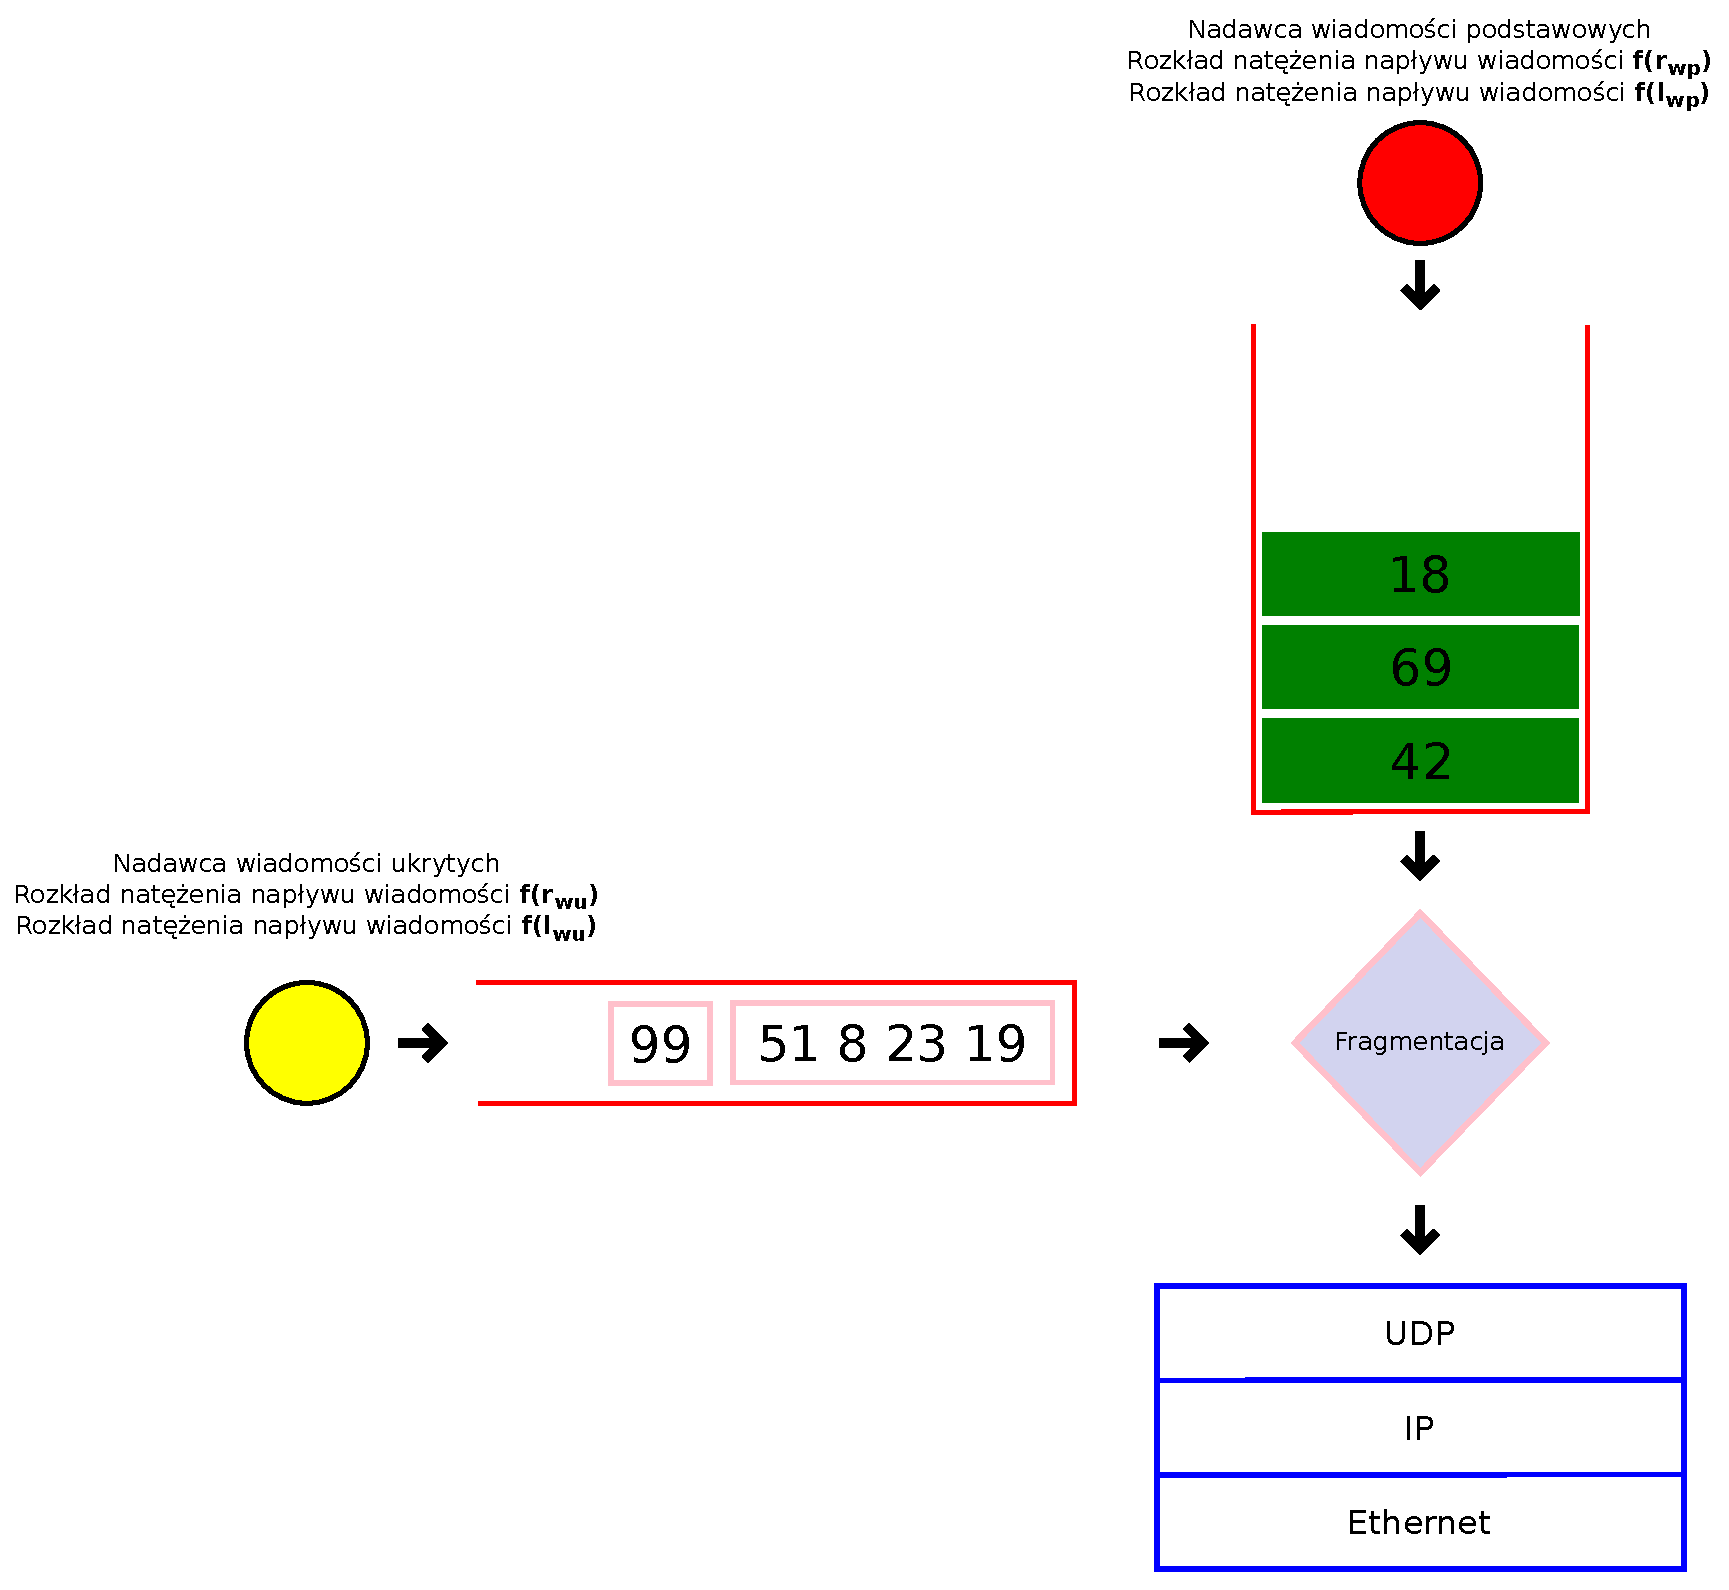
\includegraphics[scale=0.99]{hidden_channel_model}
            \caption{Model kanału ukrytego}
            \label{HIDDENCHANNELMODEL}
    \end{figure}

    \section{Założenia i ograniczenia projektowe}
    W czasie projektowania protokołu a następnie jego badań przyjęto następujące założenia:
    \begin{enumerate}
        \item \emph{Pojemność kolejki wiadomości ukrytych i podstawowych jest nieograniczona} -
            jak zostanie omówione w następnym rozdziale, działanie protokołu
            kanału ukrytego wymaga kolejkowania zarówno wiadomości podstawowych
            jak i ukrytych, w obecnej wersji protokół kanału ukrytego nie wspiera
            żadnego mechanizmu radzenia sobie z przeciążeniami, w związku z tym
            dla ułatwienia prowadzenia badań założono nieskończoną pojemność obu kolejek

        \item \emph{Wiadomość(zarówno podstawową jak i ukrytą) traktujemy, jako odebraną,
            gdy wszystkie jej segmenty zostaną odebrane przez odbiornik} - jak powiedziano
            wcześniej, wiadomości ukryte mogą składać się z więcej niż jednego segmentu,
            natomiast jak zostanie powiedziane, wiadomości podstawowe mogą być fragmentowane
            w celu transmisji pakietów z ukrytymi wiadomościami, aby umożliwić
            obliczanie opóźnień zarówno wiadomości podstawowych jak i ukrytych,
            zakłada się, że opóźnienie to czas pomiędzy napłynięciem wiadomości,
            a odebraniem ostatniego jej segmentu

        \item \emph{Komunikacja pomiędzy odbiorcą a nadawcą odbywa się bez błędów transmisji} -
            jak wspomniano wcześniej, protokół UDP jest protokołem zawodnym, również
            zaprojektowany protokół kanału ukrytego nie zapewnia mechanizmów niezawodnej
            transmisji danych, w zawiązku z czym, aby nie komplikować metodologii
            obliczania opóźnień poszczególnych wiadomości, związanych z utratą
            pakietów je transportujących, założono, że w trakcie transmisji nie
            występują żadne błędy, zarówno podstawieniowe jak i wtrąceniowe

        \item \emph{Długość wiadomości ukrytej musi być wielokrotnością długości segmentu
            wiadomości ukrytej (DSWU)} - długość każdego odebranego przez odbiorcę pakietu,
            jest przez niego interpretowana jako wartość segmentu danych ukrytych o określonej
            długości, w związku z tym konieczne jest zapewnienie, że wszystkie segmenty
            wiadomości ukrytej są tej samej długości i są w pełni wypełnione, co czasami
            wymaga zastosowania dopełnienia, przyjęcie tego założenie upraszcza protokół
            kanału ukrytego, ponieważ odpowiedzialność za dopełnienie wiadomości ukrytych
            spada na użytkownika kanału
    \end{enumerate}
    \section{Słownik używanych pojęć}
    \begin{itemize}
        \item \emph{Kanał podstawowy(nośnik)} - kanał, w którym zarówno fakt transmisji,
            jak również treść przesyłanych danych, jest widoczna dla osób postronnych,
            wykorzystywany do realizacji kanału ukrytego

        \item \emph{Wiadomość podstawowa (WP)} - wiadomość transmitowana kanałem
            podstawowym

        \item \emph{Kolejka wiadomości podstawowych( \( K_{WP} \) )} - kolejka, w
                której przechowywane są, ze względu na brak możliwości natychmiastowej
                transmisji, wiadomości podstawowe, jednostką pojemności kolejki
                wiadomości podstawowych jest bajt

        \item \emph{Kanał ukryty} - kanał umożliwiający transmisje danych w taki sposób,
            aby osoba postronna obserwująca kanał transmisyjny nie była świadoma
            nie tylko treści wiadomości, ale również faktu, że transmisja wiadomości ma miejsce

        \item \emph{Wiadomość ukryta (WU)} - wiadomość transmitowana kanałem ukrytym

        \item \emph{Kolejka wiadomości ukrytych ( \( K_{WU} \) )} - kolejka, w
                której przechowywane są, ze względu na brak możliwości natychmiastowej
                transmisji, wiadomości ukryte, jednostką pojemności kolejki
                wiadomości podstawowych jest bit

        \item \emph{Segment wiadomości ukrytej (SWU)} - fragment, porcja danych
            wiadomości ukrytej, które transmitowane są (w sposób ukryty) w jednym
            pakiecie przesyłanym za pomocą protokołu usługowego

        \item \emph{Długość segmentu wiadomości ukrytej \( D_{SWU} \)} - liczba
                bitów zawartych w jednym segmencie danych ukrytych

        \item \emph{Wartość segmentu wiadomości ukrytej \( W_{SWU} \)} - wartość
            liczbowa segmentu wiadomości ukrytej potraktowanego, jako liczba binarna,
            na przykład dla segmentu wiadomości ukrytej o treści 11010011:
            \( W_{SWU}(11010011) = 211 \)

       \item \emph{Maksymalna wartość segmentu wiadomości ukrytej (\( Max_{W_{SWU}} \))} -
           maksymalna wartość, jaką może przyjąć segment wiadomości ukrytej przy
           założonej wartości długości segmentu wiadomości ukrytej, czyli wartość
           segmentu wiadomości ukrytej, w którym wszystkie bity mają wartość 1,
           na przykład dla \( D_{SWU} = 8 \), segment o wartości maksymalnej to
           \( 11111111 \), a jego wartość to: \( Max_{W_{SWU}} = 255 \)

       \item \emph{Fragmentacja pakietów} - procedura podziału jednego pakietu na
           kilka mniejszych na przykład w celu równoważenia obciążenia poprzez
           wysłanie mniejszych pakietów różnymi trasami

       \item \emph{Agregacja pakietów} - procedura syntezy większego pakietu z
           kilku małych pakietów na przykład w celu optymalizacji stosunku długości
           nagłówka pakietu do długości danych

       \item \emph{Błąd transmisji} - zjawisko polegające na odebraniu przez odbiorcę
           pakietu lub segmentu zawierającego inną treść niż została w nim
           umieszczona przez nadawcę, wyróżniamy błędy podstawieniowe, które
           zmieniają wartość pojedynczych bitów wiadomości, lub błedy wtrąceniowe,
           które powodują utratę, lub odbiór większej ilości bitów niż wysłał nadawca

    \end{itemize}
    \section{Opis parametrów kanału ukrytego}
    Przykładowa komunikacja przy pomocy kanału ukrytego wygląda następująco:
        \begin{figure}[h]
                \centering
                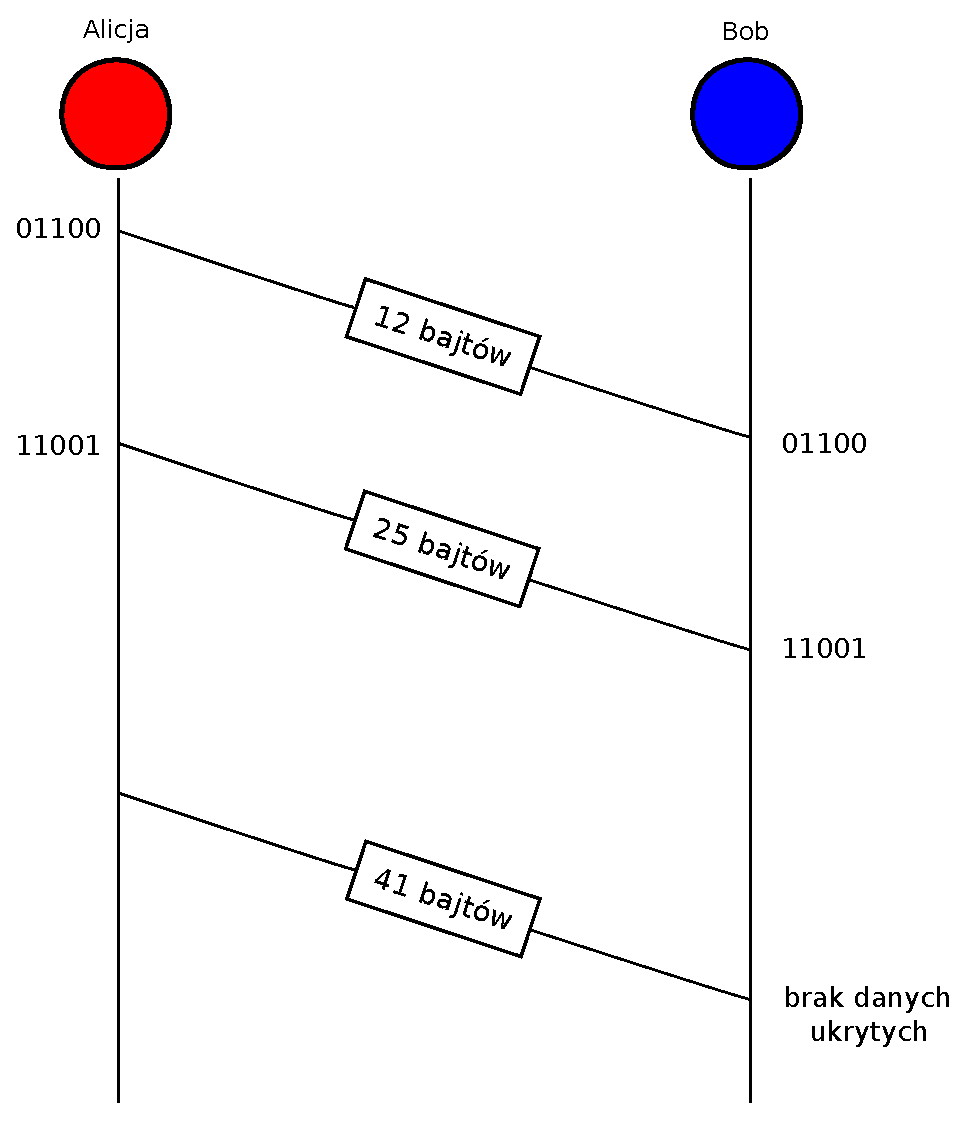
\includegraphics{komunikacja_kanalem_ukrytym_gotowa}
                \caption{Przykładowa komunikacja kanałem ukrytym}
                \label{COMMUNICATION}
        \end{figure}

    \section{Opis działania protokołu kanału ukrytego}
    \section{Schemat działania protokołu kanału ukrytego}

\chapter{Badania optymalnych parametrów i jakości kanału ukrytego}
    \section{Zależność opóźnienia wiadomości ukrytych od natężenia napływu wiadomości podstawowych}
        \subsection{Metodologia i cel badania}
        \subsection{Obserwacje}
        \subsection{Wnioski}

    \section{Zależność opóźnienia wiadomości podstawowych od natężenia napływu wiadomości ukrytych}
        \subsection{Metodologia i cel badania}
        \subsection{Obserwacje}
        \subsection{Wnioski}

    \section{Zależność opóźnienia wiadomości podstawowych od natężenia napływu wiadomości podstawowych}
        \subsection{Metodologia i cel badania}
        \subsection{Obserwacje}
        \subsection{Wnioski}


\chapter{Analiza wykrywalności kanału ukrytego}
    \section{Analiza ingerencji kanału ukrytego w kanał podstawowy}
    \section{Metody ataku na kanał ukryty}
    \section{Sugestie doboru parametrów kanału ukrytego} \label{SUGESTIEPARAMETROW}
    \section{Inne sposoby obrony przed wykryciem}

\chapter{Podsumowanie i wnioski}
\chapter{Możliwości rozwoju i kontynuacji prac}

\clearpage
\addcontentsline{toc}{chapter}{Bibliografia}
\bibliographystyle{plain}
\bibliography{bibliografia}


\end{document}
